\chapter{开发流程}
  \label{chap:开发流程}

% \section{总体开发流程}
%   \label{sec:总体开发流程}
%     本次的项目采用 AngularJS 框架开发,AngularJS 项目一般由入口页、模板、控制器、路由控制以及静态资源几大模块构成。大体而流程是: 路由配置 -> 模板设计 -> 数据构造 -> 控制器配置,这些模块的编写没有严格的顺序,模块间是由关联的,因此,改动了一个模块,其他关联的而模块都要跟着改动,下面就简单介绍一下各流程所做的工作。

%     \subsection{项目结构}
%       \label{subsec:项目结构}
%         整个项目的目录结构及如下:
%         \begin{verbatim}
%           aystore
%            |
%            |---css/ // CSS 静态资源
%            |    |---artdetail.css
%            |    |---artlist.css
%            |    |---botbar.css
%            |    ...
%            |
%            |---img/ // 主要是一些图标
%            |    |---alipay.png
%            |    |---home.jpg
%            |    ...
%            |
%            |---less // less 文件,用于编译成 CSS
%            |---node_modules // 项目用到的模块, 如 AngularJS
%            |---res // 存放一些资料,如设计图,方案规划等,不属于项目
%            |---tpl // 模板文件
%            |    |---artdetail.html
%            |    |---ayculture.html
%            |    |---pay.html
%            |    ...
%            |---app.js   // 控制器入口,路由控制,控制器代码
%            |---index.js // 视图入口,html 基本结构,静态资源的一次性引入
%         \end{verbatim}
%         \par
%         css 目录是样式目录,用来控制页面的样式;img 目录放置了 html 文件中用到的所有的图标;less 目录是存放的 less 文件,要编译成 css 文件才能执行,我采用了 Sublime 的一个插件 Less2Css,使用时他会调用 lessc 引擎,在 Less 文件保存时可以自动将其编译为 css 文件到指定目录,非常高效。node_modules 文件夹存放了项目所需的库,由 npm 包管理工具下载的库或框架都放在 node_modules 文件夹下。res 文件夹存放了资料,例如项目规划、设计图等,不属于项目组成;tpl 文件夹存放了模板文件,对应于 MVC 模型中的 view, 由控制器控制路由与填充数据。入口页 index.html 负责引入页面的基本框架、静态资源以及视图入口。这是 SPA 应用的模式,详见 \ref{subsubsec:spa}。app.js 是控制逻辑的入口页,包含了路由的配置及各个模板的控制器。

%     \subsection{路由配置}
%       \label{subsec:路由配置}
%         路由的机制我们在 \ref{subsubsec:ui_router_模块} 简要介绍过,我把项目中的路由划分为了两个部分,一个是包含底部菜单的路由,另一个是没有底部菜单的路由。有底部菜单的路由都设置成某个父路由的子路由,父路由的代码如下:
%         \begin{lstlisting}
%           $stateProvider
%             .state('main', {
%               url: '/main',
%               templateUrl: "tpl/main.html",
%               views: {
%                 '': {
%                   templateUrl: "tpl/main.html"
%                 },
%                 'content@main': {
%                    templateUrl: "tpl/home.html"
%                 },
%                 'botmenu@main': {
%                    templateUrl: "tpl/botmenu.html"
%                 },
%               }
%             })
%         \end{lstlisting}
%           上面的代码是主路由(或者叫父路由)的配置,state() 方法的第一个参数为状态名,或者叫路由名; 第二个参数是一个对象,url 字段表示 "main" 这个路由的路径,templateUrl 表示显示的页面文件,此页面文件的作用是划分视图,这里划分为两个视图,一个对应主要内容,另一个对应底部菜单。继承了 "main" 这个路由的子路由继承了 "main" 的整个模板,包括底部菜单与内容部分,然后只需修改 content 的部分就可以实现子路由的视图。

%     \subsection{模板与样式设计}
%       \label{subsec:模板与样式设计}
%         一个模板就是一个页面,只不过很简洁,只有关键的 html 代码,而没有外部文件引入、页面头的设置等,如图 \ref{fig:tpl1}, 这就是前面提到的 SPA (单页应用)的特性,详见 \ref{subsubsec:spa} 一节。
%         \begin{figure}[H]
%           \centering
%           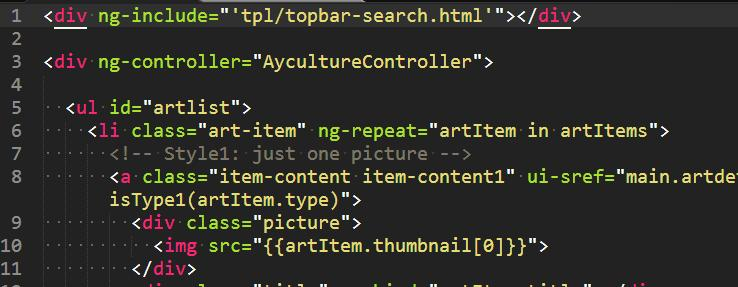
\includegraphics[width=8cm]{./img/tpl.jpg}
%           \caption{简洁的模板页}
%           \label{fig:tpl1}
%         \end{figure}
%         模板的主要作用是展现页面,因此要和配合 CSS 的控制。SPA 应用的样式需要考虑命名空间的问题,因为所有的 CSS 文件都是一次性引入的,如图 \ref{fig:css}
%         \begin{figure}[H]
%           \centering
%           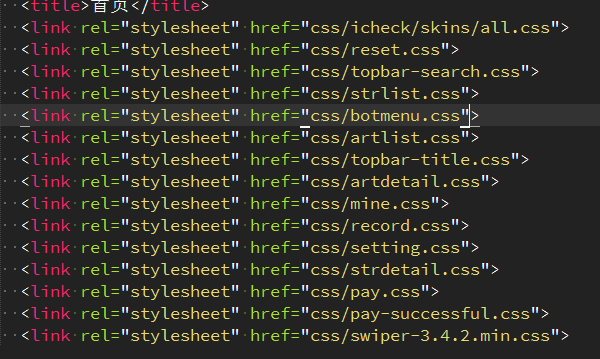
\includegraphics[width=10cm]{./img/css.png}
%           \caption{一次性引入所有的 CSS 样式}
%           \label{fig:css}
%         \end{figure}
%         我个人的处理方法是:对于每个 CSS 文件,用一个和文件名一样的容器把样式包裹起来,当然,我直接编辑的仍是 Less 文件,像这样 \ref{fig:wrapper},而且用 ID 而不是 Class 来确保唯一性, 让每个CSS 有自己的作用域,这个灵感来自于 AngularJS 的控制器的作用域,把每个模板的数据封闭起来,很好的避免了冲突。
%         \begin{figure}[H]
%           \centering
%           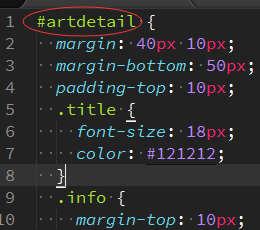
\includegraphics[width=5cm]{./img/wrapper.png}
%           \caption{用 Wrapper 包裹起整个 Less 文件}
%           \label{fig:wrapper}
%         \end{figure}

%     \subsection{数据与逻辑业务}
%       \label{subsec:数据与逻辑业务}
%         数据部分是前端设计中很重要的一环,个人认为,前端的设计大体分为两大块内容,一个是样式的设计,一个是数据与逻辑业务。好的样式设计需要花很长的时间,因为应用越精美,需要调的细节就越多,但 CSS 并不是一门语言,他只是个属性库而已,通过一点一点叠加样式实现想要的效果,没有深入的概念,没有更高的抽象的层次;而数据部分,更多地涉及逻辑,属于 JavaScript 部分,是编程,是语言,这就需要开发者有着很强的 JavaScript 语言基础,尤其是 DOM 和 BOM 对象,掌握一门语言是要花很长时间的,大量的而应用才能更深入的理解本质,例如 JavaScript 的一些核心概念:原型、继承、对象等,如果理解不够深入,编写的代码就可能冗杂、难以维护。尤其在用框架的时候,框架固然简单,可以大大简化代码,但是缺点是这是别人的东西,自己不理解原理,实现相同功能的 API 有很多,但其实用到的是同一段核心代码,此时与其去记忆那么多方法,不如深入挖掘代码,理解本质,这样才能走得更远。

%     \subsection{控制器设计}
%       \label{subsec:控制器设计}
%         控制器的作用,个人通过写代码的理解,主要作用是指挥,指挥模型与模板,指挥数据朝哪走,例如:路由控制、请求控制,根据URL调用哪个页面以及获得 HTTP 请求后,把请求送给谁(某个服务)处理,控制器中不推荐写业务逻辑、数据的具体处理。
%         \par
%         控制器在两个地方设置,模板文件中的引入,用来控制作用范围,js 文件中的定义与具体逻辑实现。我的项目中,每个模板页的主要内容都用一个控制器包裹起来,如图 \ref{fig:ctrl},
%         \begin{figure}[H]
%           \centering
%           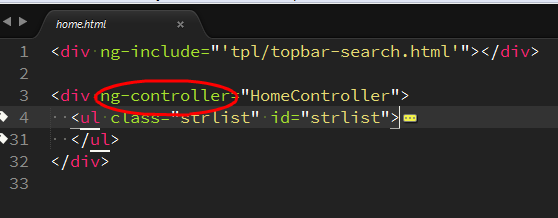
\includegraphics[width=8cm]{./img/ctrl.png}
%           \caption{模板中的控制器声明 }
%           \label{fig:ctrl}
%         \end{figure}
%         其他的地方是代码片段的包含,用其他的控制器设置,也就是说,控制器只是控制一部分 html 片段,让代码片段间的数据隔离,因此,一个页面是可以被多个控制器同时控制的,多个页面的某部分也可以由一个控制器来控制,例如底部菜单的部分,好几个页面都有,甚至有的页面一个控制器也没有,例如视图页,只放两行代码,用于模板的插入,此机制是由 ui-router 实现的,详见 \ref{subsubsec:ui_router_模块}。
%         \par
%         控制器的 js 代码放在了 app.js 文件中,,如图 \ref{fig:ctrl_js}
%         \begin{figure}[H]
%           \centering
%           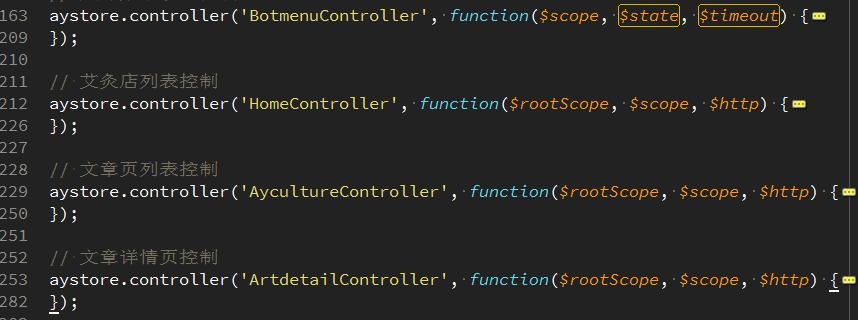
\includegraphics[width=12cm]{./img/ctrl_js.png}
%           \caption{app.js 中的控制器}
%           \label{fig:ctrl_js}
%         \end{figure}
%         此文件放置了所有的控制器代码以及路由配置,后面会讲到。

%         \par
%         以上的步骤没有严格而顺序,因为各部分会相互关联,例如:修改模板的 HTML 结构时,样式文件也要跟着修改很多,因此,各个过程几乎是同时进行的。接下来我挑选一些代表性的页面来讲解我的设计流程。这些页面有的用到了 AngularJS 的重要概念,如服务,有的囊括了业务逻辑技术难点,有的包含了重要的数据构造。

\section{home 页的设计}
  \label{sec:home_页的设计}
    \subsection{功能分析}
      \label{subsec:功能分析}
        首页的设计图 \ref{fig:home}:
        \begin{figure}[H]
          \centering
          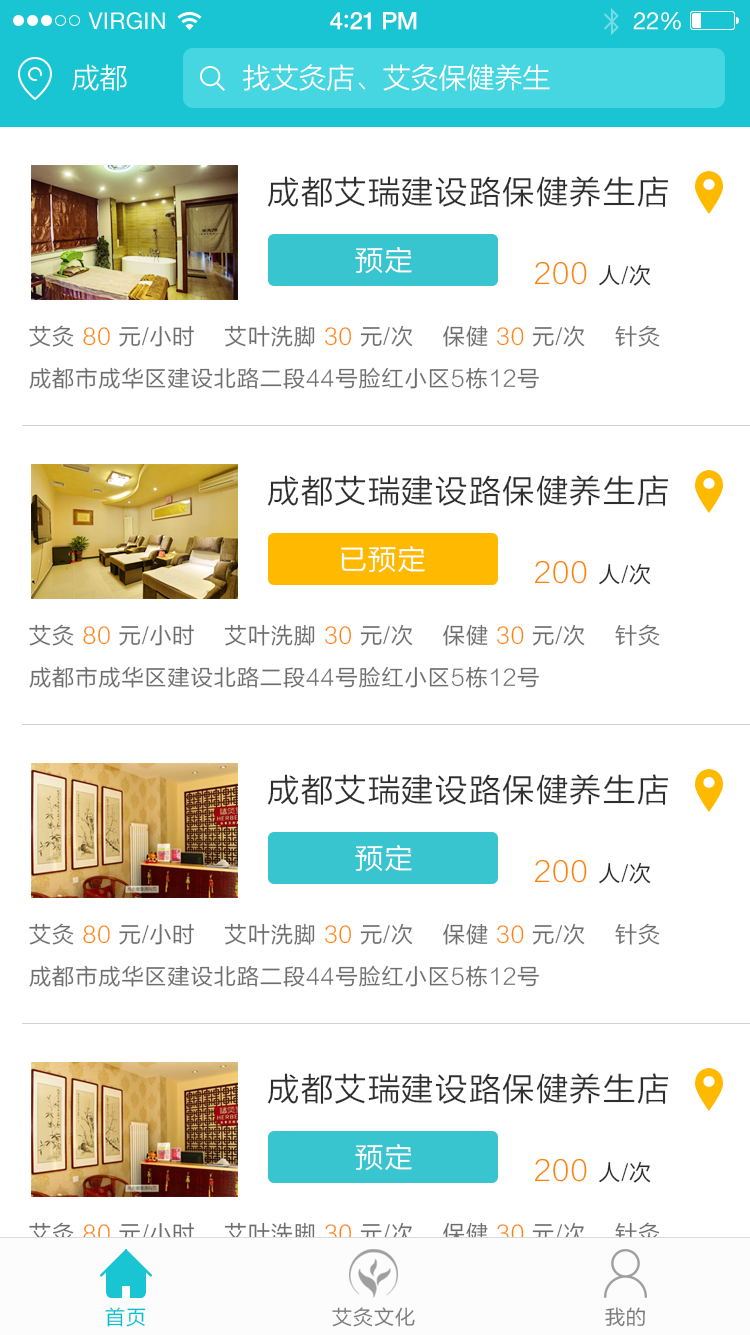
\includegraphics[width=8cm]{img/201705181050.jpg}
          \caption{首页设计图}
          \label{fig:home}
        \end{figure}
        首页主要用来加载从服务器返回的 json 数据并以列表呈现, 数据的填充用到了 AngularJS 的模板渲染引擎,语法简洁,功能强大,不只是 home 页,其他的页面也都用到了此功能。 Home 页的设计难点不多,本节主要是来介绍 AngularJS 的命令与模板引擎的使用以及数据的构造。

    \subsection{数据设计}
      \label{subsec:数据设计}
        根据设计图 \ref{fig:home},列表中的每一项展示了如下的信息:
        \begin{itemize}
          \item 缩略图
          \item 店名
          \item 预定状态
          \item 艾灸保健价格
          \item 其他各项服务与价格
          \item 详细地址
        \end{itemize}
        于是我们可以构建如下的 JSON 数据,模拟从数据库提取的数据:
        \begin{lstlisting}
          [
              {
                "strId": "123",// 店的 ID
                "strCity": "成都",// 城市
                "strDistrict": "成华区",// 市区
                "strThumbnail": "http://i2.muimg.com/589268/8aefeb670174ad96t.jpg",// 缩略图
                "strName": "成都艾瑞建设路保健养生店",// 店名
                "ordStatus": 0,// 预定状态,0:已预订,1:未预定
                "strLink": "strlink/store1.html",// todo
                "avgPrice": 200,// 艾灸服务价格
                "srvInfo": "专业技术服务提供服务,智能艾灸床 5 张,艾灸、刮痧、洗脚、按摩、保健、亚健康、养生。",// 描述
                "full": 0,// 是否满员
                // 其他服务的信息
                "strServices": [
                  {
                    "srvName": "艾灸",// 服务名
                    "srvPrice": 80,// 服务价格
                    "srvUnit": "元/小时"// 价格单位
                  },
                  {
                    "srvName": "艾叶洗脚",
                    "srvPrice": 30,
                    "srvUnit": "元/次"
                  },
                  {
                    "srvName": "针灸",
                    "srvPrice": "",
                    "srvUnit": ""
                  }
                ],
                "strMap": "",// todo
                "strAddress": "建设北路二段44号脸红小区5栋12号"// 详细地址
              },
              {
                  "strId": "123",
                  "strCity": "成都",
                  "strDistrict": "成华区",
                  ...
              },
              ...
          ]
        \end{lstlisting}
        缩略图字段是调用的外部的链接,我把图片放到了专门的图片服务器上存储,这样可以节约服务器的空间,这样服务器上不需要再单独开辟一个文件夹盛放图片,也省去了给图片命名的麻烦,也能防止误删、图片文件夹改名的操作导致的图片链接失效。我采用的图片服务器是 “贴图库”,网址为:\url{http://www.tietuku.com/}, 网站虽然样式粗糙,但功能上考虑地很周到,例如可以给图片分组,方便管理,而且可以一键生成图片外链(包括缩略图),点击相应的按钮即可,如图 \ref{fig:tietuku}
        \begin{figure}[H]
          \centering
          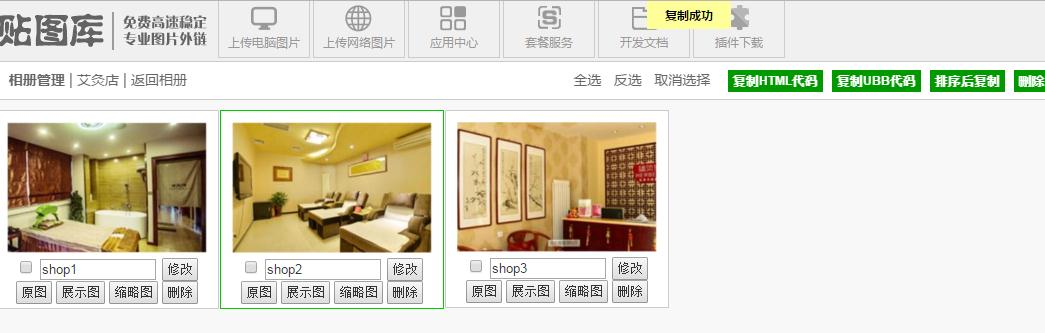
\includegraphics[width=10cm]{./img/tietuku.jpg}
          \caption{贴图库}
          \label{fig:tietuku}
        \end{figure}

    \subsection{控制器,路由}
      \label{subsec:控制器_路由}
        \textbf{路由设计}\, 路由在前面讨论过,是指将 URL 与对应的模板关联起来,而且 AngularJS 支持模板继承与视图嵌套,在路由的配置上相当强大,详见 \ref{subsubsec:ui_router_模块} 一节。商城列表页的设计图 \ref{fig:home} 底部有控制菜单,根据前面的提到的,应该作为 "main" 路由的子路由,然后,只需修改 "content" 视图。代码如下:
        \begin{lstlisting}
          .state('main.home', {// 商城页视图
            url: '/home',
            views: {
              'content@main': {
                 templateUrl: "tpl/home.html"
              }
            }
          })
        \end{lstlisting}
        路由配置好后还要引入,不过不是通过通常的 "href" 标签,而是 "ui-sref=stateName", 即状态名,状态名即路由的标识,支持点操作符的继承操作,这个前面有提到。
        \par
        \textbf{控制器设计}\, 控制器的使用比较简单,如前面提到的,分成两个部分,一个是模板中的引入,一个是 app.js 中的详细实现,这里再简要说一下,后面其他页的设计不再过多叙述。
        \par
        控制器引入。控制器在模板中用 ng-controller=HomeController 命令括住一个(标签)范围,这样就可以将各个控制器隔开,隔离变量的作用域。
        \par
        变量模板。变量可以在 html 标签中用某种语法直接引入,这是使用框架的优势之一。变量在 html 中直接用 {{}} 括起来即可,或者用 ng-bind=varName 命令,这两个命令有一点差别,{{}} 相对于 ng-bind 写起来简便,不会额外增加标签属性,导致标签的长度过长,但是有时刷新过快会导致出现 "{{item}}" 这种情况,但极为少见,因此项目中多采用这种方式,我把这种方式暂且成为变量模板。变量模板支持还支持 "." 操作符,即访问对象的 key 。
        \par
        重复命令 ng-repeat。商城页部分主要是列表展现,列表的特点是重复,文章页也是类似,每个 item 都有相同的数据结构,在数据上是一个数组,AngularJS 提供了方便的 ng-repeat 命令可以很容易地解决此问题,写法为:
        ng-repeat="item in items", 类似 "for in" 循环。
        \par
        更强的 class 命令——"ng-class"。根据设计图 \ref{fig:home}, 我们看到有一个人性化的功能,预订过的店面会把按钮变成黄色而不是蓝色,同时改变按钮的文本为"已预订"。这个功能 AngularJS 很容易实现,AngularJS 允许在 html 标签中加入简单的的逻辑,当然复杂的最好写在控制器中,更复杂的写在服务中。ng-class 命令和 ng-bind 命令都支持这样一种语法,{val1:'str1', val2:'str2', ...}[val], 类似于 switch 命令,根据后面的值去选择相应的 class 或者标签内容,因此这里只需 ng-class="{0:'btn-blue', 1:'ordered'}[strItem.ordStatus]" 和 ng-bind="{0:'预定', 1:'已预订'}[strItem.ordStatus]" 这两个命令即可实现。
        \par
        域——\$scope 和 全局域——\$rootScope。上面谈到的都是模板中的命令,接下来说说 js 代码中的控制器如何写。控制器有自己的域——\$scope,域的意思是作用范围,是一个对象,变量要想在控制器中使用,必须要挂载到 \$scope 上。
        \par
        依赖注入与服务。前面提到,控制器 controller 在使用时需要两个参数,控制器的名字和一个回调函数,而后面的回调函数的参数引入是 AngularJS 的一大特色——依赖注入机制。我们知道,一般的函数参数是有顺序的,要省略只能省略后面的几个,顺序弄反结果结果就不正确。而 AngularJS 的回调函数的参数引入根本不需要考虑顺序,只要名字写对即可,因为 AngularJS 是根据名字检测的,这样用起来就很简单,用什么参数就放什么参数即可,只不过这些参数在 AngularJS 中称为服务 (Service),这就是依赖注入机制——Dependency Injection。而服务指的是一些对象,有自己的方法和属性,与一般的对象不同的是,服务是 AngularJS 的一个概念而已,用来在控制器间传递数据的,定义一个服务,在任何控制器中都能引入(依赖注入)。这里用到的服务是 \$http、\$scope 和 \$rootScope。\$http 是用来发送 ajax 请求的,用于从服务器上获取数据。\$scope 和 \$rootScope 前面提到过,是作用域,变量向模板传递的通道。
        \par
        最终,home 页的控制器代码如下:
        \begin{lstlisting}
          // 艾灸店列表控制
          aystore.controller('HomeController', function($rootScope, $scope, $http) {
            $http.get('data/strlist.json', {
                params: {
                  "custId": "12323",
                  "data": "strList"
                },
                responseType: "json"
              })
              .then(function(res) {
                console.log(res.data.data);
                $rootScope.strItems = res.data.data;
              }, function() {
                alert('error');
              });
          });
        \end{lstlisting}
        可以看到,代码十分简洁,因为 home 页没有什么逻辑,而数据也是提前组织好的,组成一个大对象挂载到 \$scope 上,而不是把对象拆开,一个一个把 key 挂到 \$scope 上,其实这就是我之前的做法,组成一个对象的方法是我探索的,这样让控制器更简洁,大大简化代码量。

    \subsection{home 页最终效果}
      \label{subsec:home_页最终效果}
        最终实现的效果如 \ref{fig:home1}
        \begin{figure}[H]
          \centering
          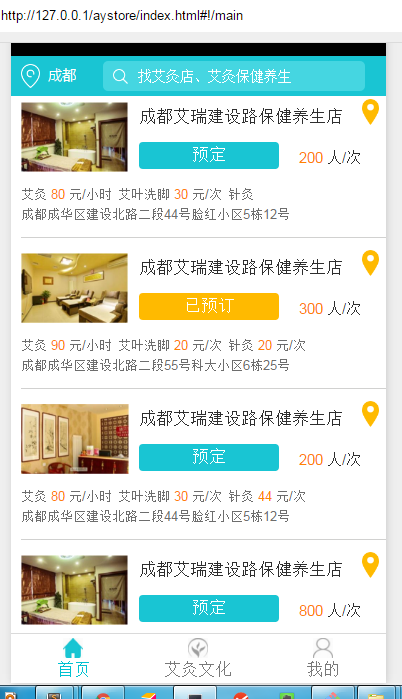
\includegraphics[width=8cm]{./img/home1.png}
          \caption{home 页的实际效果}
          \label{fig:home1}
        \end{figure}
        可以看到,和设计图基本一样,其实数据是核心,这里展示的只是样式效果,是 CSS 的功劳。

\section{strdetail 页的设计}
  \label{sec:strdetail_页的设计}
    strdetail 是指店铺的详情页,这一页用于展示店铺的内部,用于服务的预定于下单等。设计图如 \ref{fig:strdetail}
    \begin{figure}[H]
      \centering
      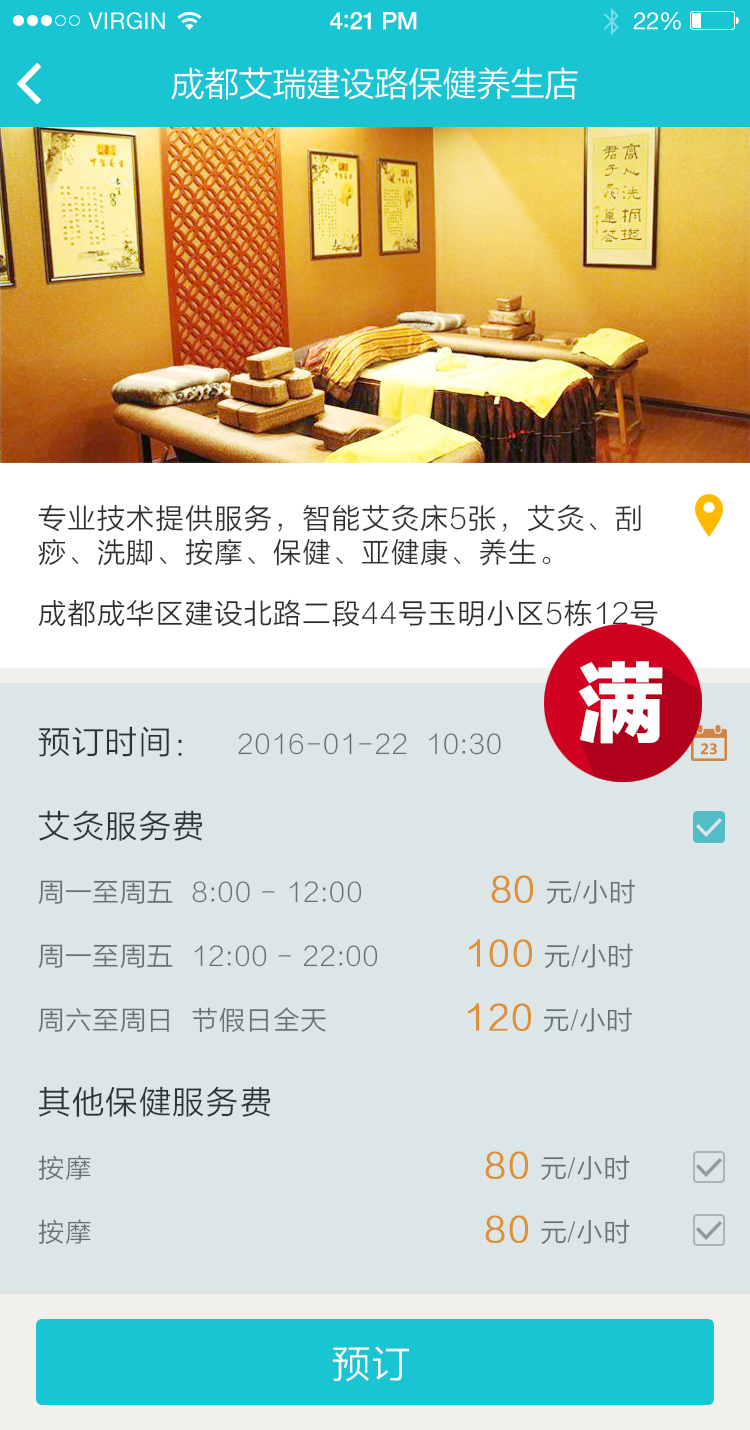
\includegraphics[width=10cm]{./img/strdetail.png}
      \caption{店铺详情页设计图}
      \label{fig:strdetail}
    \end{figure}

    \subsection{需求分析}
      \label{subsec:需求分析}
        这一页要实现的功能是服务选择或者说是订单填写,订单的填写共有两页,这一页选择服务,下一页选择人数。这一页的服务选择共需选择三个参数:时间、主服务与其他服务。单击预定时间右边的日期图标可以选择日期。主服务这里指的就是艾灸服务费,主服务费不同时间有不同的价格,这里有代码逻辑可以自动计算,其他的服务不用多说,按需勾选即可,因为其他的服务费比较低,都是一些辅助性服务,因此不需要根据特别是的定制特别的价格,那样反而增加了麻烦度。

    \subsection{设计难点剖析}
      \label{subsec:设计难点剖析}
        这一页以及下一页是订单的填写,是一个商城系统的重要部分,主要是负责购物车逻辑,要提交你保存的商品以及件数。设计的难点主要存在以下方面:
        \begin{itemize}
          \item 订单格式与填写
          \item 根据时段确定价格的逻辑
        \end{itemize}
        而且既然要通过两页填写订单,还存在一个页面间传输信息的问题,对于 AngularJS 来说,就是控制器之间的数据传输问题。以下就来详细介绍设计过程。

    \subsection{POST 数据构造}
      \label{subsec:post_数据构造}
        作为商城的购物车逻辑,需要哪些数据?大体逻辑是:谁在什么时候买了什么商品,各买了多少件,当然这里的商品不是实在的商品,而是服务,服务要携带时间信息,即你什么时候接受服务,"谁"指的是客户的基本信息,包括其 id,手机号等,服务信息要保存服务名、服务的人数、服务的价格,价格不是必须的,因为防止客户在本地蹿改,价格要在服务器真正计算,本地的计算是为了实时显示。我构造的数据如下:
        \begin{lstlisting}
          // 订单数据管理
          var order = {
            'ordId': 'adafdfefdvefsdvsd1213',
            'creTime': new Date().getTime(),
            'custId': 'sjdkfjsdfweioje12',
            'phone': 1234567,
            'srvTime': '',
            'aySrv': {
              'inputName': "ay",
              'name': '艾灸床保健',
              'price': 0,
              'num': 0
            },
            'othSrv': []
          };
        \end{lstlisting}
        参数以及解释如 \ref{tab:orderdata}
        \begin{table}[htbp]
          \caption{订单数据构造}
          \label{tab:orderdata}
          \centering

          \begin{tabular}{rl}
          \toprule
          字段名 & 解释 \\
          \midrule
          ordId     & 订单编号 \\
          creTime   & 下单时间 \\
          custId    & 客户编号 \\
          phone     & 客户手机号 \\
          srvTime   & 服务的时间 \\
          aySrv     & 艾灸服务,即主服务,是一个对象 \\
          inputName & 服务名字代号,用于构建表单的 name \\
          name      & 服务名字,中文名 \\
          price     & 价格 \\
          num       & 数量 \\
          othSrv    & 其他服务,是一个数组\\
          \bottomrule
          \end{tabular}
        \end{table}

        othSrv 指其他服务,是一个数组,每个对象也都有 inputName, name, price 和 num 四个参数。

    \subsection{日期选择的逻辑}
      \label{subsec:日期选择的逻辑}
        这一页有个设计难点,根据设计图 \ref{fig:strdetail} ,艾灸服务的价格在不同时间是不一样的,在用户构造订单的时候可以自动计算,那么时间段如何表示呢?比如周一到周五、周一和周三、8:00-12:00 这些时间段如何表示,如何解析?我的设计思想如下。
        \par
        日期的表示。日期的字段名我定义为 weekday, 格式规则定义如下:
        \par
        \begin{itemize}
          \item 用包含数字(1-7)、逗号(","")和分割线("-") 的字符串表示 weekday (周几)
          \item 数字 1-7 分别表示周一到周日
          \item 逗号表示不连续
          \item 分隔符表示连续
          \item 可以很好地处理空格
        \end{itemize}
        举例:如 "1 - 5" 表示周一到周五,"1, 2-4, 5-7" 表示周一、周二至周四、周五至周日,语法简单,非常方便。
        \par
        时间的表示。时间的表示更简单,"08:00-12:00" 就表示 08:00 到 12:00。
        \par
        日期和时间的判断。把时间和日期表示出来后,接下来就是如何判断选择的日期在哪个区间,然后自动确定价格。首先要获取填写的订单的时间(是享受服务的时间,不是下单时间),是在日期选择栏中,用 jquery 获取日期和时间,是一个字符串,如: "2017-05-18 19:46:28",接下来是分别提取日期和时间,利用 split(" ") 方法可以在空格处将一个字符串分割成字符串数组,上面的字符串被分割成一个包含日期的字符串和一个时间字符串,接下来带入日期和时间的判断服务中判断,复合要求的写入订单。流程图见 \ref{fig:DateAndTime}
        \begin{figure}[H]
          \centering
          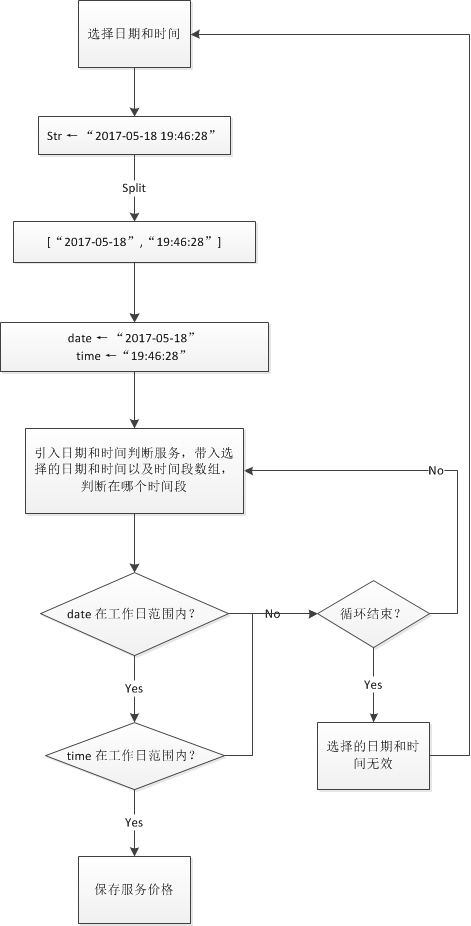
\includegraphics[width=12cm]{./img/DateAndTime.png}
          \caption{日期和时间的判断流程}
          \label{fig:DateAndTime}
        \end{figure}
        \par
        日期和时间判断的服务——DayAndTimeTest。前面介绍过,服务是 AngularJS 中用于在控制器间传递数据的一种机制,这里的数据不只是数据,也可以是方法。AngularJS 的最佳实践是在控制器中尽可能少得放置复杂的逻辑,而将他们放在服务中。图 \ref{fig:DateAndTime} 的流程中我们看到简化了的判断过程,即 date 是否在范围内和 time 是否在范围内,这里主要是调用 DayAndTimeTest 这个服务,这个服务包含两个方法,一个是日期的测试: isDayInRange(),一个是时间的测试: isTimeInRange()。
        \par
        日期判断——isDayInRange() 的实现,主要思想是如何把之前定义的日期格式字符串转化成数组,如:"1,2-5,7" -> [1, 2, 3, 4, 5, 7], 然后把选择的日期转化成工作日对应的数字,判断该数字是否在数组中, JS 没有判断元素是否在数组中的函数,因此需要自己定义,我利用了 JS 的原型特性,在原型链上直接定义方法,然后每个数组一构建就有了该方法。
        \par
        时间判断——isTimeInRange() 的实现。这里时间段不包括离散的时间段,只有一个连续的,如 "12:00-22:00",利用 split("-") 把字符串分割成两个时间点,然后判断选择的时间是否在此范围内,我的方法是把时间点转化成分钟再比较,这样比较就十分简单了。

\section{支付页的设计}
  \label{sec:支付页的设计}
    支付页的难点主要在于总价的实时变化,如图 \ref{fig:real_time_price} ,这一点
    \begin{figure}[H]
      \centering
      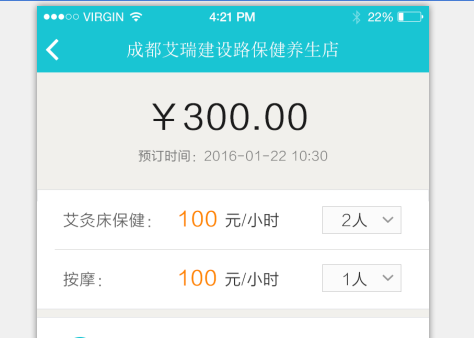
\includegraphics[width=8cm]{./img/real_time_price.png}
      \caption{总价的实时显示}
      \label{fig:real_time_price}
    \end{figure}
    当用户在下拉菜单中选择人数的时候,上面会实时显示总价。这个功能看起来简单,只是简单的 jQuery 操作,但是如果放在 AngularJS 框架中,就这存在很多问题,我在这里遇到两个严重的 bug ,这两个 bug 困扰了我几周的时间而没有任何进展,目前已经解决。
    \par
    第一个 bug 是 AngularJS 框架的 \$scope 问题,挂载到 \$scope 上的值不能实时显示,即如果我不断改变 \$scope 上的某个值,他的值不会实时显示到视图上,而是只有第一次挂载的值才可以,不过解决方案是——延时挂载,即引入一个 \$timeout 服务,类似 timeout 函数,延时挂载 \$scope 上某个值,不用设置时间,然后每次改变 \$scope 上的值后,就能实时显示。
    \par
    第二个 bug 是 DOM 操作与 AngularJS 的冲突,在上一步获得订单数据后,这一页要根据订单的项目进行页面渲染,因此是需要一定时间的,此时如果用jQuery 获取元素,然后赋值,结果竟然不变,任由我怎么选择人数,总价就是不变,后来我反复思考,查资料都没找到满意的答案,包括 Stackoverflow 上,我又去了解了 AngularJS 的原理,但实在是太深奥,我 AngularJS 用得不太熟练,原理要经过长年累月的积累才能慢慢理解。后来我又一行一行代码分析,一行一行打印,不断排除可能性,最后发觉用 jQuery 获取元素的时候输出了一个奇怪的结果,如图 \ref{fig:total_price_bug}
    \begin{figure}[H]
      \centering
      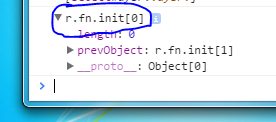
\includegraphics[width=5cm]{./img/total_price_bug.PNG}
      \caption{获取元素时的一个奇怪结果}
      \label{fig:total_price_bug}
    \end{figure}
    正常情况下,输出来的一般是类似 [select\#aysrv] 这样的结果,我一开始觉得代码有问题,我把代码直接粘到控制台运行,仍能打印结果,而且是正常的,证明获取元素的代码没问题,反反复复调了好几次,突然想到,会不会是时间上的问题,我尝试在获取元素之前加了 \$timeout 延时服务,延时3s左右,果然出了结果,我又联想到在用 jQuery 库的时候,一定要在顶部加一段代码:jQuery(document).ready(function(\$) \{ \}) 这个函数,用于文档加载完成再执行代码,最后我推断应该是页面没有渲染完,而且是因为 ng-repeat 这样的命令导致的。不管怎样,写代码不能存在侥幸,如果想走得更远,少走坑,必须深入理解框架,而这永远永远不是短时间就能掌握的,需要常年累月的积累,所以个人不相信所谓的速成教程,也不相信某些老师所说的短短两周内开发出什么,这一定是有代价的,你会忽略很多细节,没时间深入思考,躲开的困难以后一定会再次找上门来,而且会反复让你在同一个坑跌倒。

\section{底部菜单的设计}
  \label{sec:底部菜单的设计}
    底部菜单的设计体现过程中有两个问题值得探讨,一个如何用 AngularJS 的控制器控制,另一个是 AngularJS 中 jQuery 选择问题。

    \subsection{底部菜单的控制逻辑}
      \label{subsec:底部菜单的控制逻辑}
        底部菜单的控制逻辑。底部菜单的设计我是把它单独做成了路由,有自己的控制器,像之前在 \ref{subsubsec:ui_router_模块} 提到的,是某个父路由的子路由,与 content 视图分开,也就是说,在有底部菜单的页面,内容和底部菜单是分别由两个控制器控制的,这样的好处是减少代码的耦合,从而更易维护,因为整个底部菜单的控制放在单独的一个控制器下,而不是分散到各个页面的控制其
    \subsection{jQuery 的选择问题}
      \label{subsec:jquery_的选择问题}
        Misco Hevery 曾在一次访谈谈到,他设计 AngularJS 初衷是用 html 标签构建应用,通过给 HTML 标签扩展属性和定义新的标签,配合控制器的控制就可以轻松、方便地构建应用(其实一点都不轻松,如果不熟练的话)。但是如果要涉及到复杂的dom操作,AngularJS 就无能为力了,因为 AngularJS 的 DOM 操作很弱,每个操作都要插入到标签上,这仿佛又回到了以前大量采用嵌入css样式控制页面样式的时代,一种相当烂的设计原则,这个时候 jQuery 就会发挥作用,很好地弥补了这一缺陷,底部菜单的控制主要是根据不同页面,把菜单的文字和图标高亮显示,提示客户所处的栏目,这一点用jQuery 就很好实现,而用 AngularJS 本身的 ng-show 来绑定样式就很复杂。因此,我们在构建AngularJS 应用时,要注意 jQuery 的取舍,不要大量依赖,也不要完全抛弃,AngularJS 和 jQuery 在很多时候是互补的。

\section{本章小结}
  \label{sec:开发流程小结}
    本章主要讨论了 AngularJS 项目的开发流程,结合设计过程穿插介绍了 AngularJS 的一些重要概念以及具体应用,重点放在了数据构造问题以及设计重点难点上,而没有详细地讨论每一页的设计。
    \par
    再谈一点对 AngularJS 与构建项目的感想。一个项目的构建离不开那几个流程:需求分析-设计-实现,当然,实际的过程更复杂,还要包括系统的测试反馈过程。AngularJS 作为一款重量级的框架,给构建应用提供了很多方便,当然也给调试带来了巨大的困难,要想熟练地用好框架,要不断提高自己的调试技能,深入应用的每个流程,花时间深入理解框架,遇到问题多去深入思考解决,而不是为了追求快速而去逃避问题。
